% Resumen de resultados en inglés (guía, sección 6, entregable 3). Una página; figuras en la segunda.
% Los números salen de results.json a través de valores_E1.tex (macro V); no se escriben a mano.
\documentclass[10pt,a4paper]{article}
\usepackage[T1]{fontenc}
\usepackage[utf8]{inputenc}
\usepackage{lmodern}
\usepackage[english]{babel}
\usepackage[margin=1.9cm]{geometry}
\usepackage{microtype}
\usepackage{amsmath,amssymb}
\usepackage{graphicx}
\usepackage{booktabs,array}
\usepackage[hidelinks]{hyperref}
\graphicspath{{../figuras/}}
\setlength{\parindent}{0pt}
\setlength{\parskip}{4pt}
\pagestyle{empty}
% Generado automáticamente por generar_results.m desde results.json (clave valores_informe). No editar a mano.
\providecommand{\V}[1]{\ifcsname val@#1\endcsname\csname val@#1\endcsname\else\textbf{??\detokenize{#1}??}\fi}
\expandafter\def\csname val@m_A_kit\endcsname{1.8\times10^{-16}}
\expandafter\def\csname val@m_A_jac\endcsname{9.0\times10^{-13}}
\expandafter\def\csname val@m_polo_e\endcsname{-7240.6}
\expandafter\def\csname val@m_sep_polo\endcsname{411}
\expandafter\def\csname val@m_EL\endcsname{2.0\times10^{-16}}
\expandafter\def\csname val@p1_MF_margin\endcsname{65.5292}
\expandafter\def\csname val@p1_MF_margin_dif\endcsname{1\times10^{-3}}
\expandafter\def\csname val@p1_GM_margin\endcsname{0.4142}
\expandafter\def\csname val@p1_err_escalar\endcsname{2.2\times10^{-16}}
\expandafter\def\csname val@p1_MF_q1\endcsname{65.5302}
\expandafter\def\csname val@p1_MF_qmin\endcsname{60.0000}
\expandafter\def\csname val@p1_gmin_qmin\endcsname{0.50000}
\expandafter\def\csname val@p2_err_kit_max\endcsname{2.4\times10^{-12}}
\expandafter\def\csname val@p2_err_icare_max\endcsname{2.4\times10^{-12}}
\expandafter\def\csname val@p2_K_vs_K0\endcsname{5.4\times10^{-14}}
\expandafter\def\csname val@p2_nk_res6\endcsname{1.7\times10^{-3}}
\expandafter\def\csname val@p2_nk_res7\endcsname{3.6\times10^{-5}}
\expandafter\def\csname val@p2_nk_res8\endcsname{1.2\times10^{-8}}
\expandafter\def\csname val@p2_nk_res9\endcsname{1.2\times10^{-15}}
\expandafter\def\csname val@e11_difmax_base\endcsname{2.5\times10^{-12}}
\expandafter\def\csname val@e11_err_ham_base\endcsname{9.6\times10^{-15}}
\expandafter\def\csname val@e11_err_schur_base\endcsname{2.4\times10^{-12}}
\expandafter\def\csname val@e11_err_nk_base\endcsname{1.0\times10^{-13}}
\expandafter\def\csname val@e11_err_schur_5est\endcsname{7.2\times10^{-9}}
\expandafter\def\csname val@e11_mineigP_5est\endcsname{7.4\times10^{-14}}
\expandafter\def\csname val@e11_err_ac_max\endcsname{5.7\times10^{-12}}
\expandafter\def\csname val@e11_err_b_max_4est\endcsname{7.6\times10^{-11}}
\expandafter\def\csname val@e12_nLinv_pend\endcsname{86}
\expandafter\def\csname val@e12_cota_max\endcsname{6.9\times10^{-10}}
\expandafter\def\csname val@e12_err_real_max\endcsname{2.4\times10^{-12}}
\expandafter\def\csname val@e12_res_max\endcsname{1.4\times10^{-13}}
\expandafter\def\csname val@e12_asim_max\endcsname{1.9\times10^{-13}}
\expandafter\def\csname val@e12_mineigP\endcsname{3.4\times10^{-4}}
\expandafter\def\csname val@e12_maxRe_cl\endcsname{-2.668}
\expandafter\def\csname val@e12_nLinv_epsmin\endcsname{7.07\times10^{5}}
\expandafter\def\csname val@e12_res_peor_epsmin\endcsname{7.1\times10^{-9}}
\expandafter\def\csname val@e12_res_azar_epsmin\endcsname{3.4\times10^{-3}}
\expandafter\def\csname val@e12_disc_min\endcsname{0.7}
\expandafter\def\csname val@e12_disc_max\endcsname{0.7}
\expandafter\def\csname val@e12_icare_epsmax\endcsname{1.8\times10^{-14}}
\expandafter\def\csname val@e12_icare_epsmin\endcsname{2.1\times10^{-6}}
\expandafter\def\csname val@e13_n_problemas\endcsname{39}
\expandafter\def\csname val@e13_ref_correccion\endcsname{3.4\times10^{-42}}
\expandafter\def\csname val@e13_P3_ham\endcsname{3.6\times10^{-9}}
\expandafter\def\csname val@e13_P3_schur\endcsname{1.2\times10^{-4}}
\expandafter\def\csname val@e13_P3_pend_ham\endcsname{-0.85}
\expandafter\def\csname val@e13_P3_pend_schur\endcsname{-1.17}
\expandafter\def\csname val@e13_F1_cifras\endcsname{12}
\expandafter\def\csname val@e13_F2_schur_smax\endcsname{3.0\times10^{-2}}
\expandafter\def\csname val@e13_F2_cifras\endcsname{14}
\expandafter\def\csname val@e13_F3_max\endcsname{2.4\times10^{-12}}
\expandafter\def\csname val@e13_condU11_peor\endcsname{4.0}
\expandafter\def\csname val@e13_nk_cociente6\endcsname{0.81}
\expandafter\def\csname val@e13_nk_cociente7\endcsname{1.03}
\expandafter\def\csname val@e13_nk_cociente8\endcsname{1.07}
\expandafter\def\csname val@e13b_F1_hambal_Rmin\endcsname{3.6\times10^{-9}}
\expandafter\def\csname val@e13b_F2_bal_peor\endcsname{1.9\times10^{-13}}
\expandafter\def\csname val@e13b_P11_schur_max\endcsname{1.1\times10^{-7}}
\expandafter\def\csname val@e13b_P11_nk_max\endcsname{2.6\times10^{-9}}
\expandafter\def\csname val@e13d_F1_N3_peor\endcsname{5.3\times10^{-8}}
\expandafter\def\csname val@e13e_F3_haz_max\endcsname{8.8\times10^{-10}}
\expandafter\def\csname val@e13e_F3_nosc_max\endcsname{8.8\times10^{-10}}
\expandafter\def\csname val@e13e_F2_haz_s5\endcsname{6.4\times10^{-5}}
\expandafter\def\csname val@e13e_F2_nosc_s5\endcsname{6.3\times10^{-5}}
\expandafter\def\csname val@e13e_F2_nosc_fallos\endcsname{1}
\expandafter\def\csname val@e13e_F1_hazSx_peor\endcsname{9.8\times10^{-14}}
\expandafter\def\csname val@e13e_F1_icare_peor\endcsname{2.6\times10^{-13}}
\expandafter\def\csname val@e13e_F2_hazSx_peor\endcsname{8.4\times10^{-15}}
\expandafter\def\csname val@e13e_F2_icare_peor\endcsname{7.4\times10^{-15}}
\expandafter\def\csname val@e13e_F3_hazSx_peor\endcsname{1.6\times10^{-14}}
\expandafter\def\csname val@e13e_F3_icare_peor\endcsname{2.0\times10^{-14}}
\expandafter\def\csname val@e13e_hazSx_peor\endcsname{9.8\times10^{-14}}
\expandafter\def\csname val@e13e_D6_2\endcsname{6\times10^{-8}}
\expandafter\def\csname val@e14_N\endcsname{625}
\expandafter\def\csname val@e14_n_estables\endcsname{625}
\expandafter\def\csname val@e14_n_nd\endcsname{625}
\expandafter\def\csname val@e14_Jth_min\endcsname{8.96\times10^{-3}}
\expandafter\def\csname val@e14_Jth_max\endcsname{2.23\times10^{2}}
\expandafter\def\csname val@e14_Jal_min\endcsname{2.03\times10^{-3}}
\expandafter\def\csname val@e14_Jal_max\endcsname{0.141}
\expandafter\def\csname val@e14_Ju_min\endcsname{1.56\times10^{-3}}
\expandafter\def\csname val@e14_Ju_max\endcsname{1.11}
\expandafter\def\csname val@e14_ok_C1\endcsname{625}
\expandafter\def\csname val@e14_ok_C2_ideal\endcsname{147}
\expandafter\def\csname val@e14_ok_C2_real\endcsname{115}
\expandafter\def\csname val@e14_ok_C2_real_sat\endcsname{101}
\expandafter\def\csname val@e14_sensor_falla\endcsname{48}
\expandafter\def\csname val@e14_cambian\endcsname{64}
\expandafter\def\csname val@e14_dif_lyap\endcsname{1.3\times10^{-9}}
\expandafter\def\csname val@e14_dif_suma\endcsname{1.9\times10^{-10}}
\expandafter\def\csname val@e14_dif_ode\endcsname{2.3\times10^{-11}}
\expandafter\def\csname val@e14_n_ode\endcsname{10}
\expandafter\def\csname val@e14_dif_solver\endcsname{8.9\times10^{-11}}
\expandafter\def\csname val@e14_base_C1_uc\endcsname{9.12}
\expandafter\def\csname val@e14_base_C2_th\endcsname{1.237}
\expandafter\def\csname val@e14_base_C2r_uc\endcsname{63.82}
\expandafter\def\csname val@e14_base_C2r_th\endcsname{1.345}
\expandafter\def\csname val@e14_spearman\endcsname{0.960}
\expandafter\def\csname val@e15_sigma_min\endcsname{0.458}
\expandafter\def\csname val@e15_fmin_desde_base\endcsname{0.9625}
\expandafter\def\csname val@e15_fmin_desde_malla\endcsname{0.9614}
\expandafter\def\csname val@e15_Jrel_semilla1\endcsname{0.961}
\expandafter\def\csname val@e15_val_Jrel\endcsname{0.9945}
\expandafter\def\csname val@e15_val_Jrel_desv\endcsname{0.019}
\expandafter\def\csname val@e15_ts_C1_max\endcsname{0.132}
\expandafter\def\csname val@e15_P2_K2_base\endcsname{182.5}
\expandafter\def\csname val@e15_P2_m_falla\endcsname{17.8}
\expandafter\def\csname val@e15_P2_K2_falla\endcsname{60}
\expandafter\def\csname val@e15b_r_th\endcsname{1.58}
\expandafter\def\csname val@e15b_r_al\endcsname{1}
\expandafter\def\csname val@e15b_Jrel_base_malla\endcsname{0.9991}
\expandafter\def\csname val@e15b_saa_Jrel\endcsname{0.9994}
\expandafter\def\csname val@e15b_saa_Jrel_desv\endcsname{0.0225}
\expandafter\def\csname val@e15b_saa_t\endcsname{0.12}
\expandafter\def\csname val@e15b_saa_mej_C1\endcsname{-1.2}
\expandafter\def\csname val@e15b_saa_t_C1\endcsname{-4.5}
\expandafter\def\csname val@e15b_saa_mej_C2\endcsname{1.5}
\expandafter\def\csname val@e15b_saa_t_C2\endcsname{45.8}
\expandafter\def\csname val@e15b_s1_mej_C1\endcsname{-8.2}
\expandafter\def\csname val@e15b_s1_mej_C3b\endcsname{5.2}
\expandafter\def\csname val@e15b_s1_t_C3b\endcsname{8.3}
\expandafter\def\csname val@e15c_piso_C1\endcsname{0.55}
\expandafter\def\csname val@e15c_piso_C2\endcsname{0.01}
\expandafter\def\csname val@e15c_piso_C3\endcsname{3.1}
\expandafter\def\csname val@e15c_piso_C3b\endcsname{0.09}
\expandafter\def\csname val@e15c_piso_ideal_max\endcsname{6\times10^{-16}}
\expandafter\def\csname val@e15d_K_lmi_vs_K0\endcsname{1.3\times10^{-4}}
\expandafter\def\csname val@e15d_J_lmi_libre\endcsname{1.000000}
\expandafter\def\csname val@e15d_costo_region\endcsname{2.5}
\expandafter\def\csname val@e15d_sigma_g\endcsname{2.939}
\expandafter\def\csname val@e15d_zeta_g\endcsname{0.885}
\expandafter\def\csname val@e15d_base_sigma\endcsname{2.668}
\expandafter\def\csname val@e15d_base_zeta\endcsname{0.742}
\expandafter\def\csname val@e15d_s4_Q\endcsname{1.18}
\expandafter\def\csname val@e15d_s4_LMI\endcsname{1.57}
\expandafter\def\csname val@e15d_s6_Q\endcsname{1.46}
\expandafter\def\csname val@e15d_s6_LMI\endcsname{2.79}
\expandafter\def\csname val@e15d_z85_Q\endcsname{1.48}
\expandafter\def\csname val@e15d_z85_LMI\endcsname{1.18}
\expandafter\def\csname val@e15d_z90_Q\endcsname{1.98}
\expandafter\def\csname val@e15d_z90_LMI\endcsname{1.25}
\expandafter\def\csname val@e15d_n_casos\endcsname{16}
\expandafter\def\csname val@e15d_n_region_ok\endcsname{16}
\expandafter\def\csname val@e15d_n_cota_ok\endcsname{16}
\expandafter\def\csname val@e15d_s4_C2_sat_ideal\endcsname{99.9}
\expandafter\def\csname val@e15d_5sem_Jrel\endcsname{0.977}
\expandafter\def\csname val@e15d_5sem_desv\endcsname{0.009}
\expandafter\def\csname val@e15d_5sem_mejora\endcsname{2.3}
\expandafter\def\csname val@e15d_val_ok\endcsname{20}
\expandafter\def\csname val@e15d_val_Jrel\endcsname{0.9982}
\expandafter\def\csname val@e15d_val_Jrel_desv\endcsname{0.0216}
\expandafter\def\csname val@e15d_val_t\endcsname{0.37}
\expandafter\def\csname val@e15d_val_mej_C1\endcsname{-6.6}
\expandafter\def\csname val@e15d_val_mej_C2\endcsname{-3.2}
\expandafter\def\csname val@e15d_val_mej_C3b\endcsname{7.6}
\expandafter\def\csname val@e16_rho\endcsname{1.635\times10^{-2}}
\expandafter\def\csname val@e16_corte_theta\endcsname{0.144}
\expandafter\def\csname val@e16_corte_alpha\endcsname{0.0377}
\expandafter\def\csname val@e16_franja\endcsname{0.055}
\expandafter\def\csname val@e16_al_emp\endcsname{0.430}
\expandafter\def\csname val@e16_rad_ideal_exito\endcsname{0.388}
\expandafter\def\csname val@e16_rad_oficial_exito\endcsname{0.378}
\expandafter\def\csname val@e16_rad_oficial_rec\endcsname{0.457}
\expandafter\def\csname val@e16_efecto_sensor\endcsname{-2.4}
\expandafter\def\csname val@e16_P1_razon_id\endcsname{11}
\expandafter\def\csname val@e16_P1_razon_of\endcsname{10}
\expandafter\def\csname val@e16_razon_min\endcsname{8.5}
\expandafter\def\csname val@e16_razon_max\endcsname{31.9}
\expandafter\def\csname val@e16_razon_med\endcsname{12.2}
\expandafter\def\csname val@e16_n_dir\endcsname{200}
\expandafter\def\csname val@e16_mc_N\endcsname{20\,000}
\expandafter\def\csname val@e16_mc_rec\endcsname{44.8}
\expandafter\def\csname val@e16_mc_exito\endcsname{34.6}
\expandafter\def\csname val@e16_C2_margen\endcsname{0.028}
\expandafter\def\csname val@e16_max_Kx\endcsname{9.996}
\expandafter\def\csname val@e16_dV_neg\endcsname{100}
\expandafter\def\csname val@e16_rango_obs\endcsname{4}
\expandafter\def\csname val@e16_in_rec\endcsname{5000}
\expandafter\def\csname val@e16_in_n\endcsname{5000}
\expandafter\def\csname val@e16_in_max_uc\endcsname{9.815}
\expandafter\def\csname val@e16_in_sat\endcsname{0}
\expandafter\def\csname val@e16_lote_coinc\endcsname{60}
\expandafter\def\csname val@e16_lote_n\endcsname{60}
\expandafter\def\csname val@e16_lote_dif\endcsname{1.5\times10^{-19}}
\expandafter\def\csname val@e16_vol_razon\endcsname{5506}
\expandafter\def\csname val@e16_radio_theta\endcsname{4.6}
\expandafter\def\csname val@esc_C2_sat\endcsname{1.9}
\expandafter\def\csname val@esc_C2_th\endcsname{1.345}


\begin{document}
\begin{center}
{\large\bfseries The Riccati equation and weight design for a saturated Furuta pendulum}\\[2pt]
{\small MT227C Modern and Optimal Control, UNI, 2026-2 --- Assignment E1 (Lab reports 3 and 4)}\\[1pt]
{\small Zamudio Salazar, J.\,O.\ and Nava Laburiano, D.\,A.\ --- Repository \texttt{MT227C-E1}, file \texttt{results.json}}
\end{center}

\textbf{Research question.} Which method for the algebraic Riccati equation is reliable for this plant,
when does it stop being reliable, and how do physical specifications translate into $(Q,R)$ with verifiable
guarantees on the nonlinear, saturated plant (Quanser QUBE-Servo 2 model, $V_{\max}=10$~V, $T_s=2$~ms,
2048-count encoders)?

\textbf{Claim 1 --- Scaling, not the algorithm, decides accuracy} (evidence cards E1.1 and E1.3).
For the baseline design the Hamiltonian-eigenvector, ordered-Schur and Newton--Kleinman solvers agree with
\texttt{icare} within $\V{e11_err_schur_base}$. Against a 40-digit reference over $\V{e13_n_problemas}$ stress problems,
unbalanced subspace methods lose up to $\V{e13_F1_cifras}$ digits for $R=10^{-8}$ and $\V{e13_F2_cifras}$ digits when the
velocity units change; balancing the Hamiltonian fixes the units but not the small-$R$ case
($\V{e13b_F1_hambal_Rmin}$), because forming $S=BR^{-1}B^\top$ already mixes scales. Our own extended-pencil solver with
\texttt{icare}'s state/input scaling reaches $\V{e13e_hazSx_peor}$ in the worst case. A prediction registered before
simulating (Schur more accurate than eigenvectors) was refuted: \texttt{eig} balances by default, \texttt{schur} does not.

\textbf{Claim 2 --- A small residual certifies a small error only if $\|\mathcal L^{-1}\|$ is moderate}
(evidence card E1.2). With $\mathcal L(X)=A_c^\top X+XA_c$, a constructed lightly damped case
($\|\mathcal L^{-1}\|=\V{e12_nLinv_epsmin}$) gives a residual of only $\V{e12_res_peor_epsmin}$ for a $1\,\%$ error in $P$. For the
pendulum $\|\mathcal L^{-1}\|=\V{e12_nLinv_pend}$, so the residual bound ($\le\V{e12_cota_max}$) does guarantee the computed
solution.

\textbf{Claim 3 --- Specifications are met by the baseline design, with a local certificate an order of magnitude
smaller than the empirical region} (evidence cards E1.4--E1.6). Of $\V{e14_N}$ Pareto-optimal LQR designs,
$\V{e15_malla_R1R4}$ satisfy decay $\sigma\ge\V{e15_sigma_min}$~s$^{-1}$, damping $\zeta\ge0.5$, $|\theta|\le\pi/2$ and at most
$5\,\%$ saturation in the large-angle scenario. A single-seed optimization overstated the gain
(winner's curse); with sample-average approximation and 20 independent seeds, the best design is not
significantly better than the baseline ($J_{rel}=\V{e15b_saa_Jrel}\pm\V{e15b_saa_Jrel_desv}$, $t=\V{e15b_saa_t}$), so the
baseline is kept. The ellipsoidal certificate ($\rho^\star=\V{e16_rho}$) covers $\V{e16_corte_alpha}$~rad on the pendulum
axis, whereas the nonlinear plant recovers from $\V{e16_al_emp}$~rad; the certified radius is $\V{e16_razon_min}$--$\V{e16_razon_max}$
times smaller (median $\V{e16_razon_med}$ over $\V{e16_n_dir}$ directions).

\begin{center}\small
\begin{tabular}{@{}l l l@{}}
\toprule
\texttt{results.json} key & Value & Note \\
\midrule
\texttt{resid\_care} & $\V{rc_ham}$, $\V{rc_schur}$, $\V{rc_nk}$ & normalized residual: eigenvectors, Schur, Newton--Kleinman \\
\texttt{K\_opt} & $[\V{K0_1}\;\;\V{K0_2}\;\;\V{K0_3}\;\;\V{K0_4}]$ & final design $=K_0$ (V/rad, V\,s/rad) \\
\texttt{eig\_cl\_opt} & $\V{cl_lento_re}\pm\V{cl_lento_im}j$, $\V{cl_rapido_re}\pm\V{cl_rapido_im}j$ & closed-loop poles (s$^{-1}$) \\
\texttt{rho\_elipse} & $\V{e16_rho}$ & certified sublevel set of $x^\top Px$ \\
\texttt{mc\_region} & $\V{e16_mc_rec}\,\%$ of $\V{e16_mc_N}$ & 4D Monte Carlo recovery fraction in the declared box \\
\texttt{C1} & $J=\V{esc_C1_J}$, $t_s=\V{esc_C1_ts}$~s & $\alpha_0=0.05$~rad, $\max|u_c|=\V{esc_C1_uc}$~V \\
\texttt{C2} & $J=\V{esc_C2_J}$, $\max|\theta|=\V{esc_C2_th}$~rad & $\alpha_0=0.35$~rad, saturated $\V{esc_C2_sat}\,\%$ of the time \\
\texttt{C3}, \texttt{C3b} & $J=\V{esc_C3_J}$, $\V{esc_C3b_J}$ & torque impulses; C3b saturated $\V{esc_C3b_sat}\,\%$ \\
\texttt{C4} & $\V{esc_C4_exito}/\V{esc_C4_n}$ successful & $\pm20\,\%$ parameters, $J=\V{esc_C4_J}\pm\V{esc_C4_J_desv}$ \\
\bottomrule
\end{tabular}
\end{center}

{\small\textbf{Reproducibility.} \texttt{run\_all} regenerates every figure, table and number (cached long Monte Carlo
runs with fixed seeds, option to recompute) and validates \texttt{results.json} with the course kit. All numbers in
this page are read from \texttt{results.json}. AI assistance (Claude) is documented attempt by attempt in the AI
annex.\par}

\clearpage
\begin{figure}[h]
\centering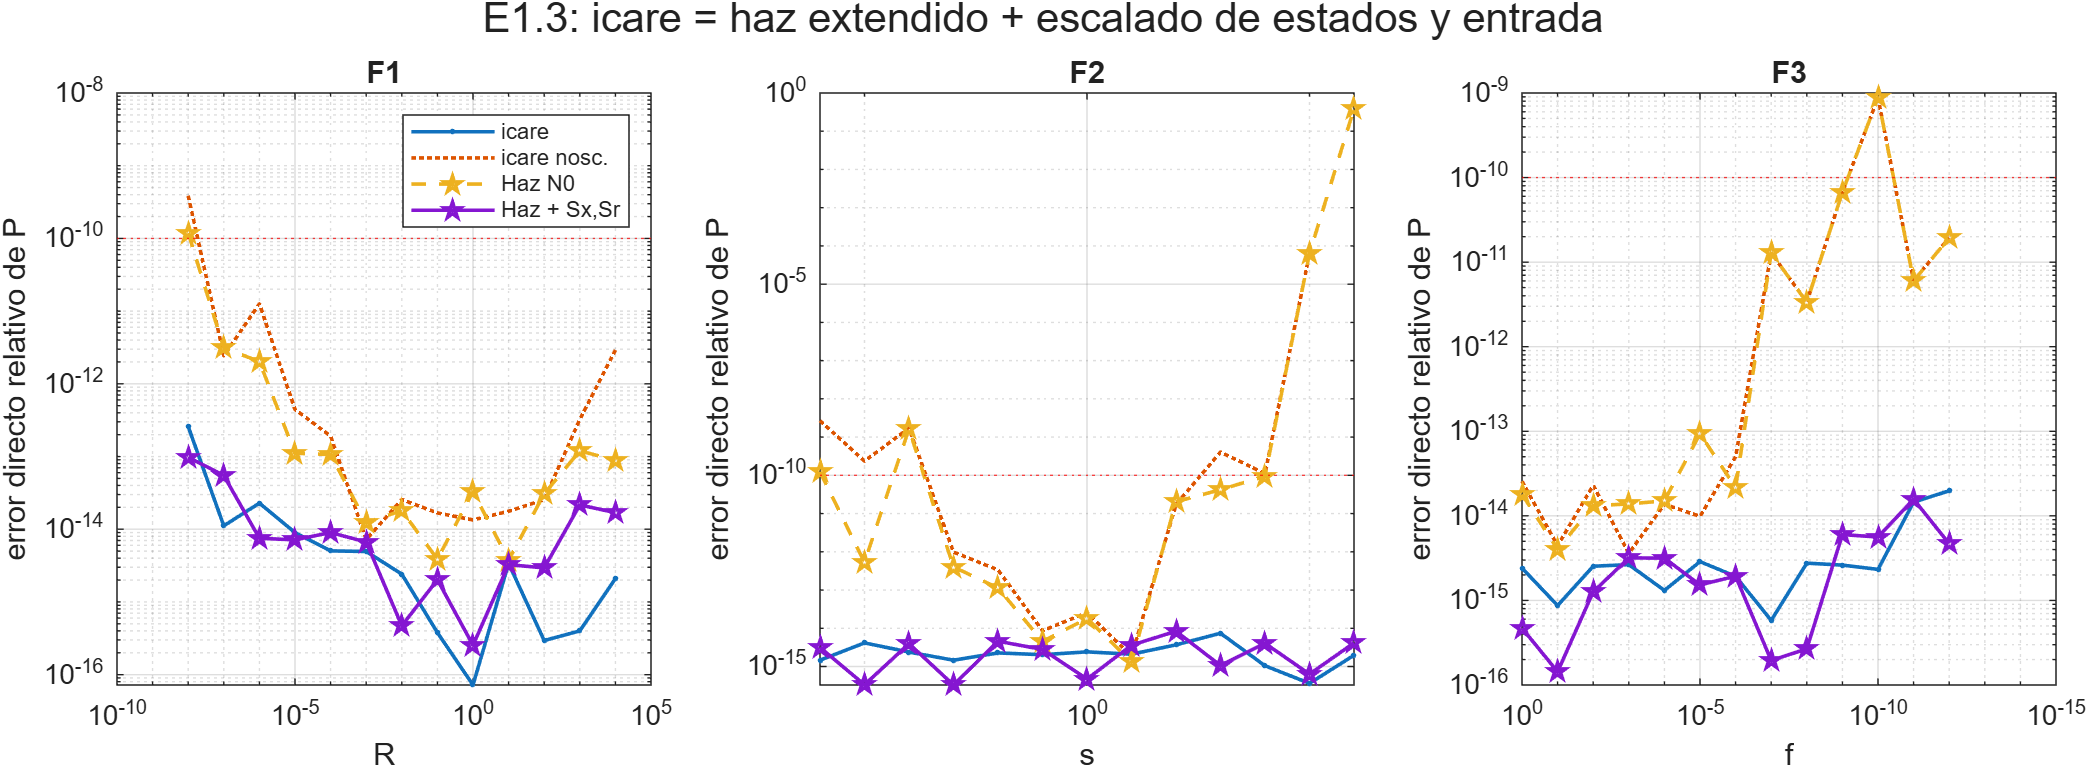
\includegraphics[width=0.95\linewidth]{E1_3_icare_escalado.png}
\caption{Claim 1. Forward error versus a 40-digit reference in the three stress families: the extended pencil
with \texttt{icare}'s scaling (``Haz + Sx, Sr'') matches \texttt{icare}; without scaling accuracy is lost.}
\end{figure}
\begin{figure}[h]
\centering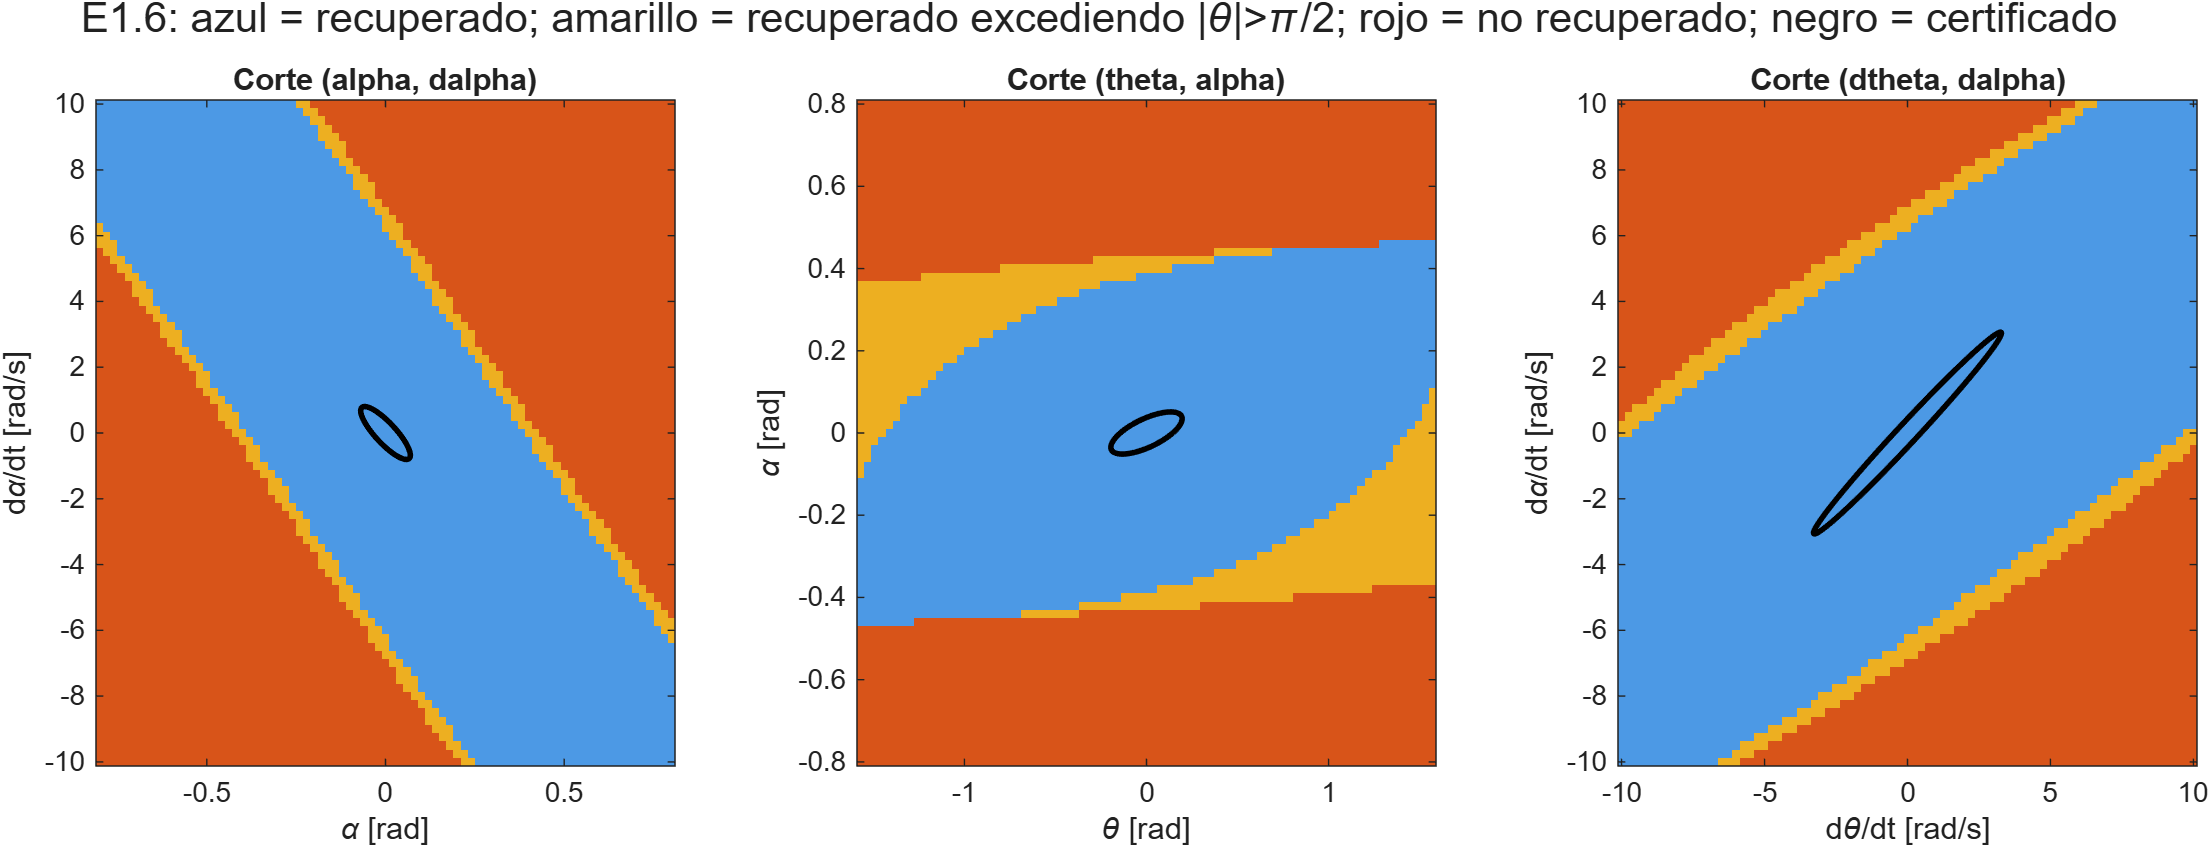
\includegraphics[width=0.95\linewidth]{E1_6_cortes.png}
\caption{Claim 3. 2D slices of the estimated region of attraction of the saturated nonlinear plant, with the
certified ellipsoid (black) superimposed.}
\end{figure}
\end{document}
